
%(BEGIN_QUESTION)
% Copyright 2008, Tony R. Kuphaldt, released under the Creative Commons Attribution License (v 1.0)
% This means you may do almost anything with this work of mine, so long as you give me proper credit

{\it Differentiator} circuits output a voltage proportional to the {\it rate of change over time} of the input voltage.  That is, the output of a differentiator circuit reflects how {\it quickly} the input voltage changes.

$$\includegraphics[width=15.5cm]{i01577x01.eps}$$

$$V_{out} = -\tau_d {dV_{in} \over dt}$$

Every differentiator circuit has a {\it time constant} ($\tau_d$), sometimes called the {\it characteristic time}, which is a proportionality constant between the input rate-of-change (measured in volts per second) and the output voltage (measured in volts).  For instance, a differentiator circuit like the one shown having a time constant of 3 seconds will output a constant voltage of -15 volts if it sees an input voltage rising at a rate of 5 volts per second:

$$-15 \hbox{ [V]} = -\left(3 \hbox{ [s]}\right) \left({5 \hbox{ [V]}\over \hbox{[s]}}\right) $$

\vskip 10pt

{\it Integrator} circuits also have time constants ($\tau_i$), expressing a proportionality between one voltage and another voltage's rate-of-change.  Explain how the time constant of an electronic integrator circuit may be calculated from component values, and then formulate a ``thought experiment'' to apply your explanation to the following integrator circuit, illustrating what the time constant means in practical terms:

$$\includegraphics[width=15.5cm]{i01577x02.eps}$$

\vskip 20pt \vbox{\hrule \hbox{\strut \vrule{} {\bf Suggestions for Socratic discussion} \vrule} \hrule}

\begin{itemize}
\item{} A useful problem-solving technique for answering qualitative or conceptual questions is to insert numerical quantities into the problem to give yourself something concrete to calculate.  Try applying this technique here.
\item{} Identify multiple ways to {\it lengthen} the time constant of either circuit.
\item{} Of those multiple ways, which do you think is easier to implement in a practical circuit?  Explain why.
\item{} Suppose a constant DC voltage signal of 2 volts was applied to the input of this integrator circuit, for a period of 1.5 seconds.  After that, the input signal goes to zero and remains there.  What will the output of this opamp circuit do, assuming it began at 0 volts before we first applied any DC input?
\item{} Assuming a constant DC voltage signal of 2 volts applied to the input of this integrator circuit, calculate all currents and voltage drops in this circuit, being sure to mark all directions of current and polarities of voltage.
\end{itemize}

\underbar{file i01577}
%(END_QUESTION)





%(BEGIN_ANSWER)

$\tau_i = RC$, just as $\tau_d = RC$ in a differentiator circuit.

$$V_{in} = -\tau_i {dV_{out} \over dt} \hbox{\hskip 40pt or \hskip 40pt} {dV_{out} \over dt} = -{V_{in} \over \tau_i} \hbox{\hskip 40pt or \hskip 40pt} V_{out} = -{1 \over {\tau_i}} \int V_{in} \> dt$$

What the ``time constant'' ($\tau_i$) means in practical terms for an integrator circuit is the amount of time it takes for the output to climb (or fall) by the amount of voltage present at the input.  Another way of saying this is that the time constant is the amount of time is takes for the circuit to {\it repeat} the input voltage.

%(END_ANSWER)





%(BEGIN_NOTES)

With $R$ = 10 k$\Omega$ and $C$ = 22 $\mu$F, the time constant for the integrator circuit will be $\tau = RC$ = 0.22 seconds.  This means if we were to input a constant DC voltage of 1 volt, the output voltage of this circuit will vary at a rate of 1 volt every 0.22 seconds, which equates to 4.5454 volts per second.

If we were to apply a 2 VDC signal to the input of this circuit, its output would linearly ramp at a rate of 9.0909 volts per second.  If this condition persisted for 1.5 seconds, the output will change a total of 13.6364 volts from where it started.  To be precise, the output will drop {\it down} 13.6364 volts from its starting point of zero, because this is an {\it inverting} opamp circuit.

\vskip 10pt

Press your students for a ``thought experiment'' of their own to illustrate what ``time constant'' means for an integrator circuit.  The point of this exercise is to get them to conceptualize the idea of ``seconds per {\it repeat''} as the integral coefficient is commonly expressed in PID controllers.












\vfil \eject

\noindent
{\bf Summary Quiz:}

Determine what the output voltage of this circuit will do when the input receives a constant DC voltage signal:

$$\includegraphics[width=15.5cm]{i01577x03.eps}$$

\begin{itemize}
\item{} The output voltage will ramp at a constant rate
\vskip 5pt 
\item{} The output voltage will decrease until it reaches zero volts
\vskip 5pt 
\item{} The output voltage will hold steady at zero volts 
\vskip 5pt 
\item{} The output voltage will ramp at an increasing rate (like a curved ski jump)
\vskip 5pt 
\item{} The output voltage will hold at a steady value equal to the input
\vskip 5pt 
\item{} The output voltage will oscillate back and forth (AC)
\end{itemize}


%INDEX% Electronics review: differentiator versus integrator circuits

%(END_NOTES)


